\documentclass[10pt,a4paper]{article}
\usepackage[utf8]{inputenc}
\usepackage[spanish]{babel}
\usepackage{amsmath}
\usepackage{amsfonts}
\usepackage{amssymb}
\usepackage{makeidx}
\usepackage{graphicx}
\usepackage[hidelinks]{hyperref}
\usepackage[left=2cm,right=2cm,top=2cm,bottom=2cm]{geometry}
\author{Ulises Isaac Reyes Alvarez\\4.B Ing. Mecatrónica\\Mtro. Carlos Enrique Morán Garabito\\"Sistemas Electrónicos de Interfaz"\\ Sep - Dic 2019}
\title{Construir un amplificación con conexión Darlington}

\begin{document}
\maketitle
\begin{figure}[hbtp]
\centering

\includegraphics[scale=2]{Pictures/UPZMG.png}
\end{figure}

\newpage
\section{Introducción}
\subsection*{Objetivos}
\begin{itemize}
\item Lograr activar el Darlington.
\item Hacer funcionar un relevador industrial con Darlington. 
\end{itemize}

\subsection*{Marco teórico}
\textbf{Transistor Darlington}\\
Frecuentemente llamado amplificador compuesto. Es una conexión muy popular de dos transistores de unión bipolar para funcionar como un solo transistor “superbeta”.La principal característica de la conexión Darlington es que el transistor compuesto actúa como una sola unidad con una ganancia de corriente que es el producto de las ganancias de corriente de dos transistores por separados.\\
Se llama transistor Darlington a la combinación de dos transistores bipolares en un tándem (al que a menudo se lo refiere como par Darlington) en un único dispositivo. La configuración fue inventada por un ingeniero de los Laboratorios Bell llamado Sidney Darlington, de ahi su nombre. La finalidad de esta configuración proporcionar un dispositivo que sea capaz de proporcionar una gran ganancia de corriente (el parámetro? del transistor). Al conseguirse comercialmente pares Darlington dentro de una misma cápsula se requiere menos espacio que si emplearemos dos transistores normales en la misma configuración.\\
La ganancia total del Darlington es el producto de la ganancia de los transistores individuales, lo que permite obtener valores muy altos, superiores a 1000. Como tiene un mayor desplazamiento de fase en altas frecuencias que un transistor único puede convertirse fácilmente en inestable.\\
\begin{figure}[hbtp]
\centering
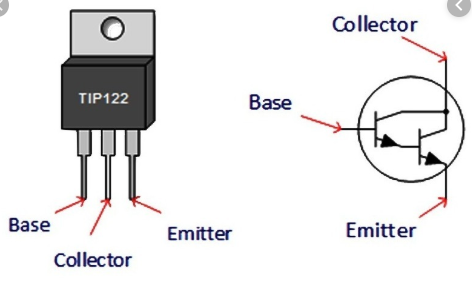
\includegraphics[scale=0.5]{Pictures/Darlington.PNG}
\caption{Estructura Transistor Darlington }
\end{figure}

\textbf{Comportamiento}\\
Esta configuración sirve para que el dispositivo sea capaz de proporcionar una gran ganancia de corriente y, al poder estar todo integrado, requiere menos espacio que dos transistores normales en la misma configuración. La ganancia total del Darlington es el producto de la ganancia de los transistores individuales.\\
Un dispositivo típico tiene una ganancia en corriente de 1000 o superior. También tiene un mayor desplazamiento de fase en altas frecuencias que un único transistor, de ahí que pueda convertirse fácilmente en inestable. La tensión base-emisor también es mayor, siendo la suma de ambas tensiones base-emisor, y para transistores de silicio es superior a 1.2V. La beta de un transistor o par darlington se halla multiplicando las de los transistores individuales. la intensidad del colector se halla multiplicando la intensidad de la base por la beta total.\\
\begin{figure}[hbtp]
\centering
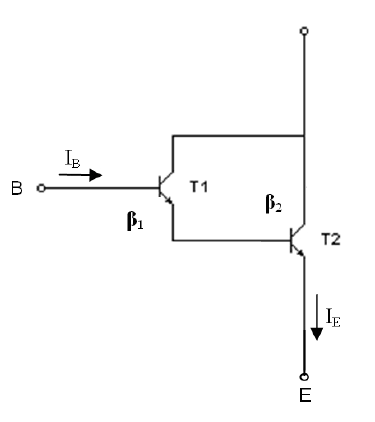
\includegraphics[scale=0.3]{Pictures/Comportamiento.PNG}
\caption{Comportamiento del Darlington}
\end{figure}

\footnote{Universidad Politécnica de la Zona Metropolitana de Guadalajara}

\newpage
\section{Materiales y equipo}
\begin{itemize}
\item Relevadores 5V / 12V
\item Protoboard
\item LED's 
\item Transitor Darlington TIP112
\item Optoacopladores 4N25
\item Push button
\item Cable para protoboard
\item Resistencias variadas
\item Fuente de alimentación para 5V, 12V y 24V
\item Caimanes 
\item Diodos 
\item LDR
\item Relevador industrial 24V
\end{itemize}

\footnote{Universidad Politécnica de la Zona Metropolitana}

\newpage
\section{Desarrollo}
\subsection{Activación del Darlington mediante Arduino y Relevador}
Para este circuito debemos utilizar el circuito de la práctica 2: \\

\begin{figure}[hbtp]
\centering
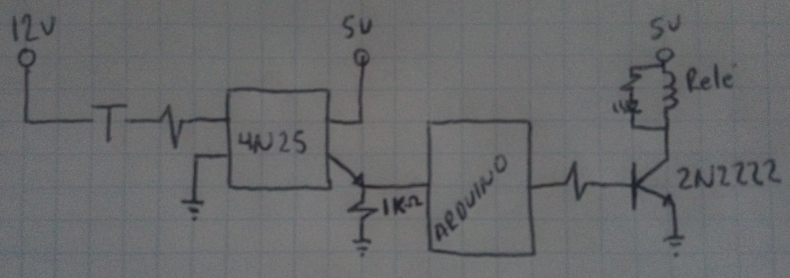
\includegraphics[scale=0.4]{Pictures/Circuito1.PNG}
\caption{Circuito práctica 2}
\end{figure}
Pero cambiamos la resistencia y el Transistor 2N2222 por el Darlington en nuestro caso TIP112, como se muestra en el siguiente circuito: 
\begin{figure}[hbtp]
\centering
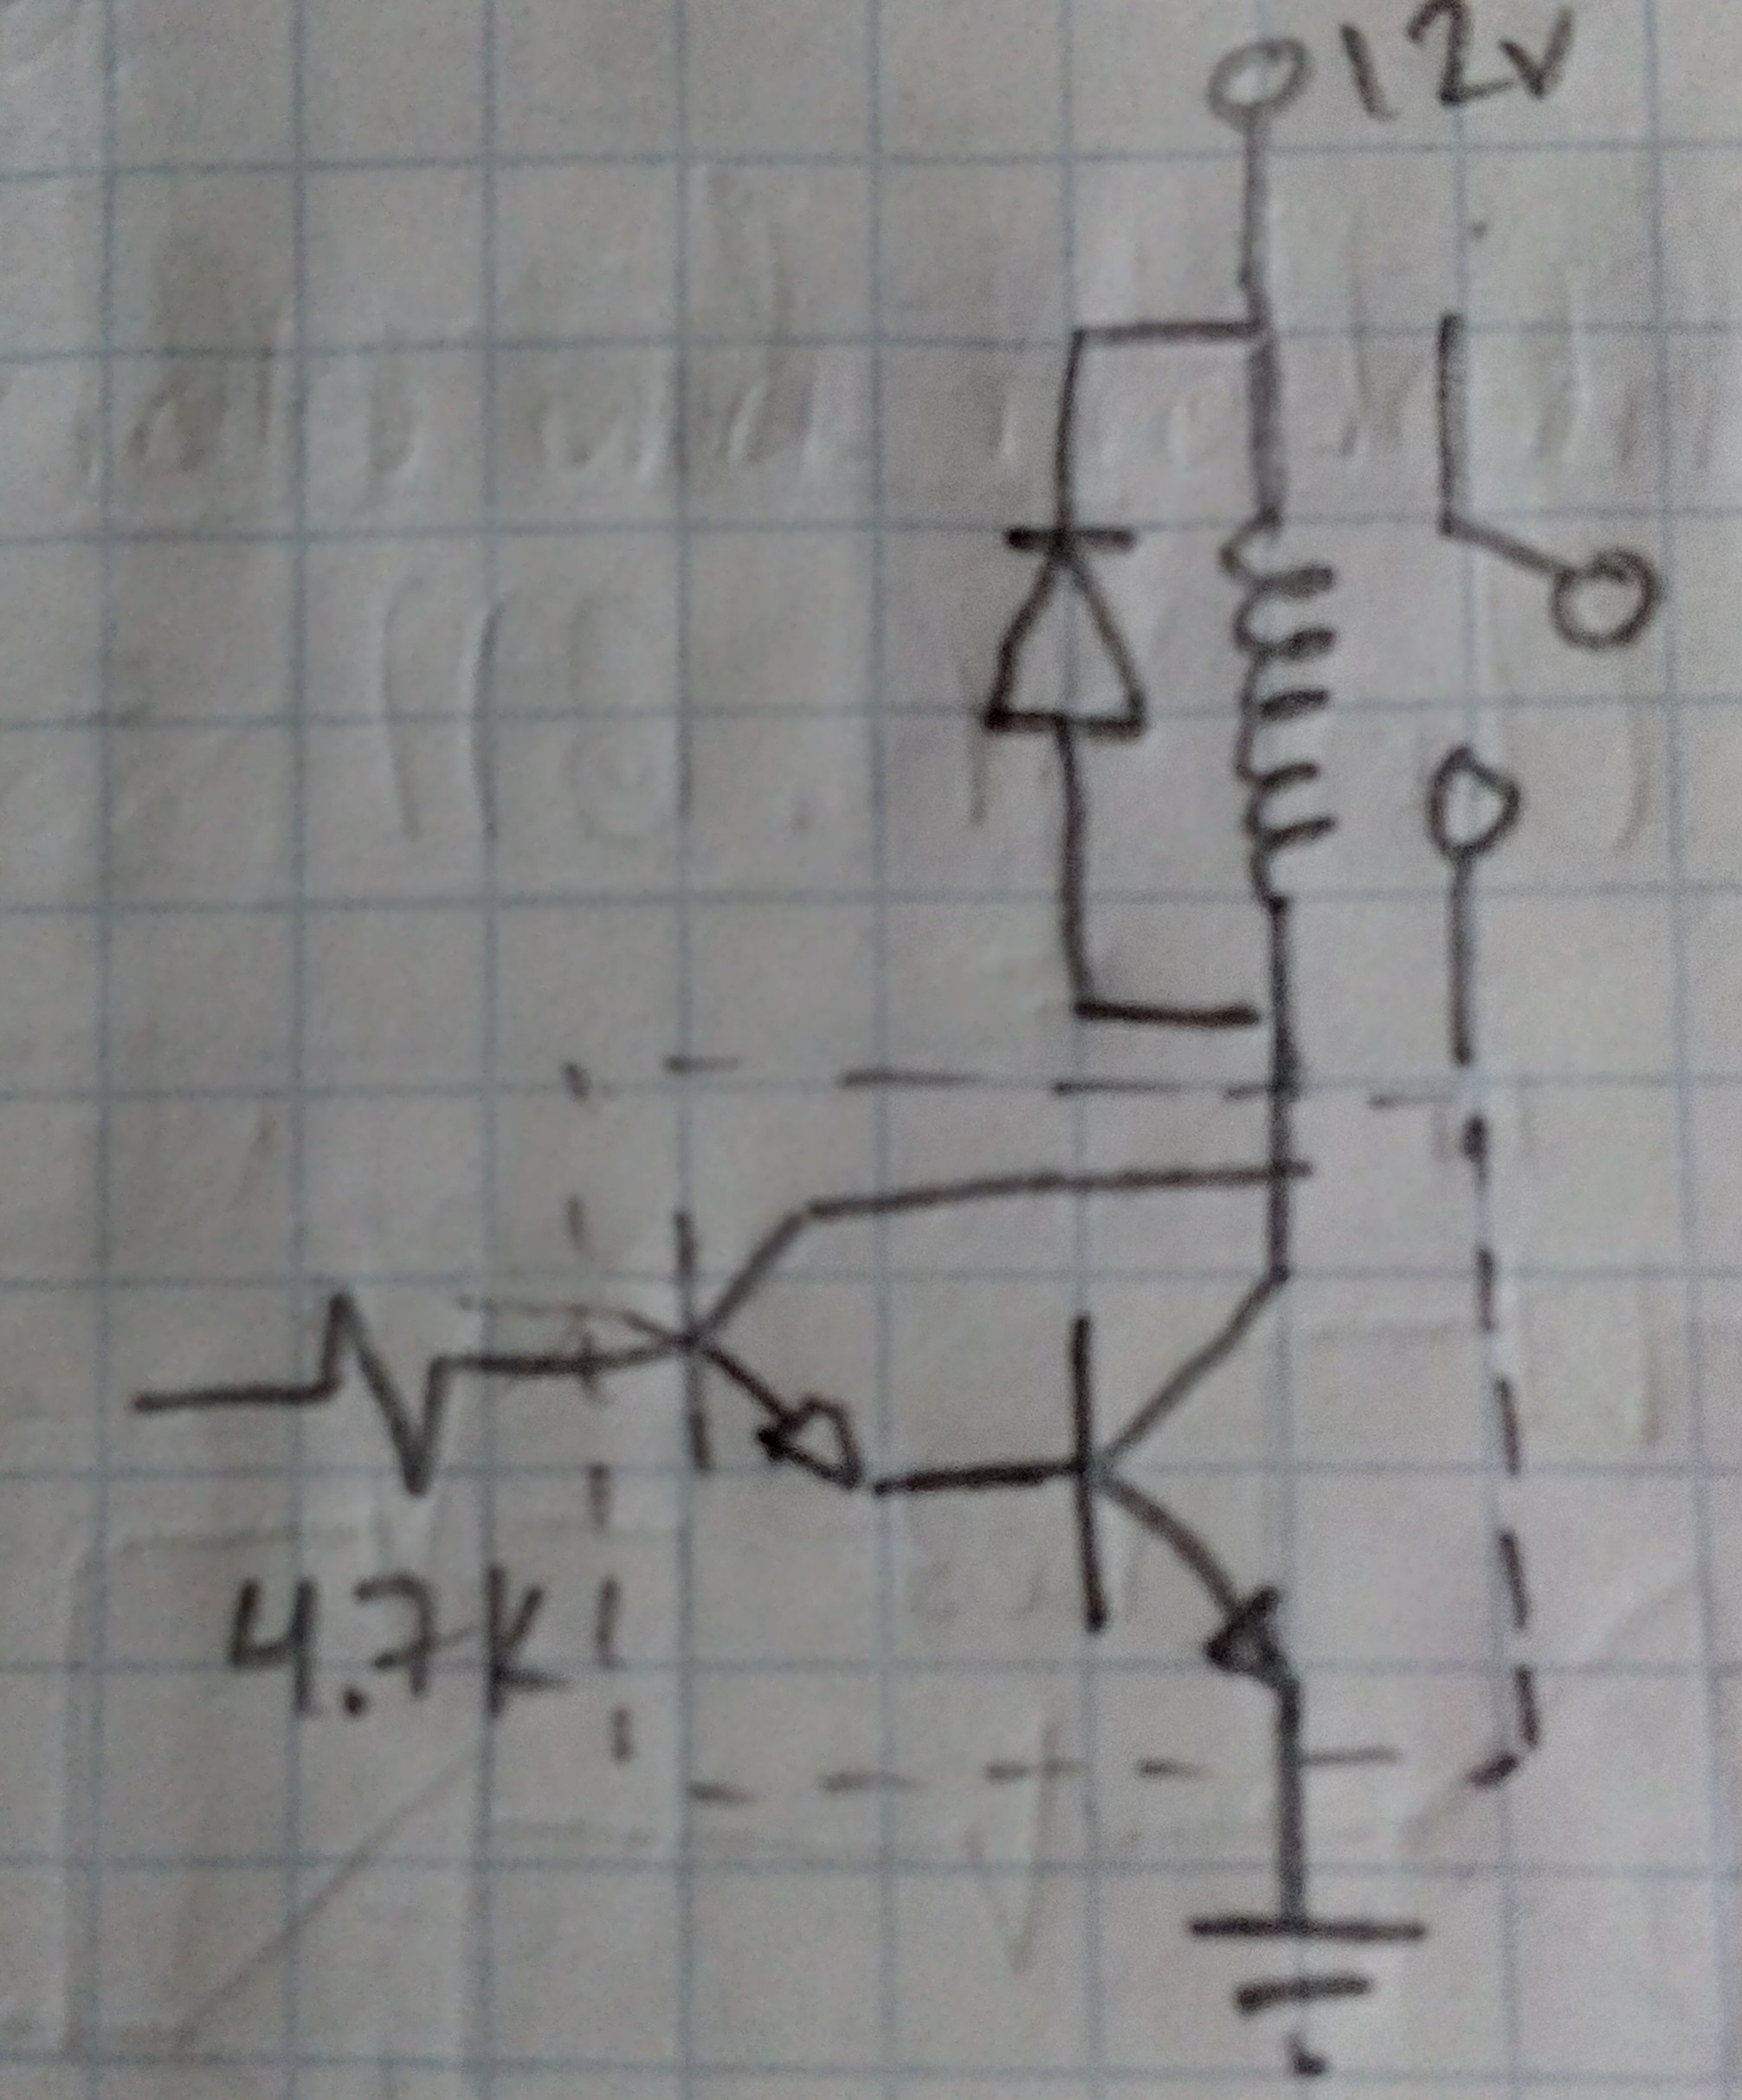
\includegraphics[scale=0.05]{Pictures/Circuito 2}
\caption{Circuito con Darlington}
\end{figure}

Armamos el circuito en Protoboard, quedando:\\
\begin{figure}[hbtp]
\centering
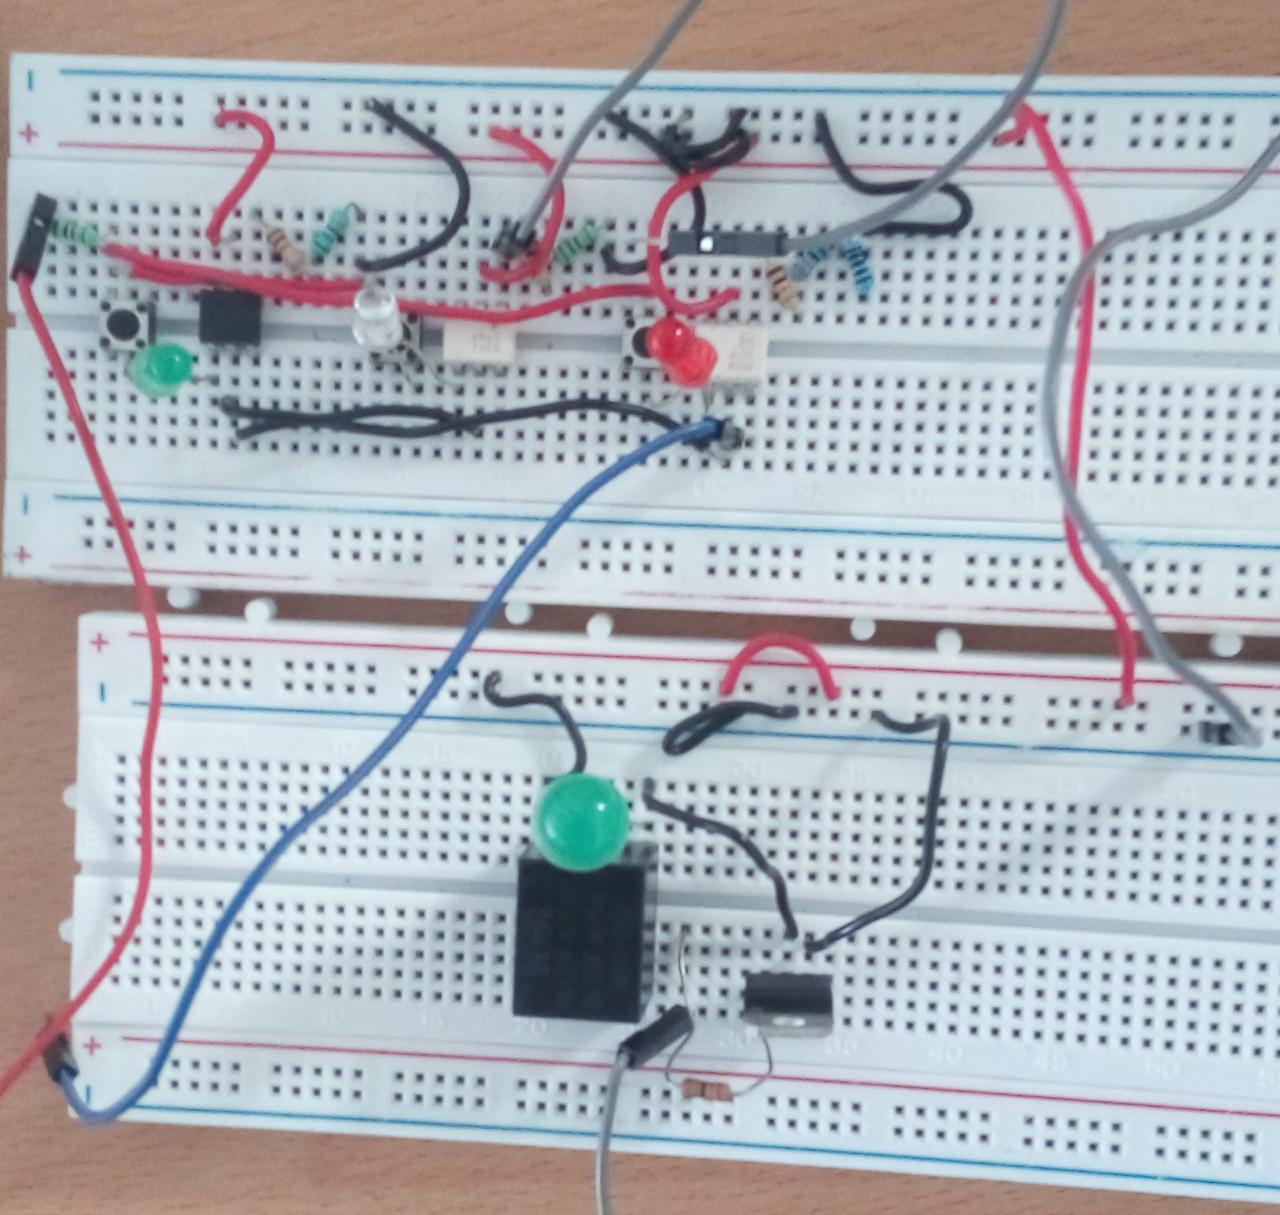
\includegraphics[scale=0.12]{Pictures/Protoboard.jpeg}
\caption{Circuito armado}
\end{figure}

Una vez armado vamos a conectar nuestras fuentes de alimentación para la activación del Darlington, teniendo una fuente de 5V para los Optoacopladores, 12V para los push button y 5V para el relavador, que puedes utilizar el mismo que utilizaste para los Optoacopladores.\\
Teniendo como resultado activación del relevador con el Darlington, mediante el arduino y código de arduino. Encendiendo el relevador y el LED para determinar que se está activando. 

\footnote{Universidad de la Zona Metropolitana de Guadalajara}

\newpage
\subsection{Activación del Darlington para activar Relevador Industrial 24V}
Para esta parte de la práctica tenemos que sustituir el relevador 5V por el relevador industrial 24V, efectivamente tenemos que también sustituir la fuente de alimentación porque si la dejamos así no nos funcionará, revisa bien tus conexiones para que todo esté correctamente y no pase nada o se queme algo.\\

Una vez echo esto debemos agregar un despeje para poder activar el Darlington, conectando otro negativo de otra fuente a la tierra de mis conexiones.\\
\begin{figure}[hbtp]
\centering
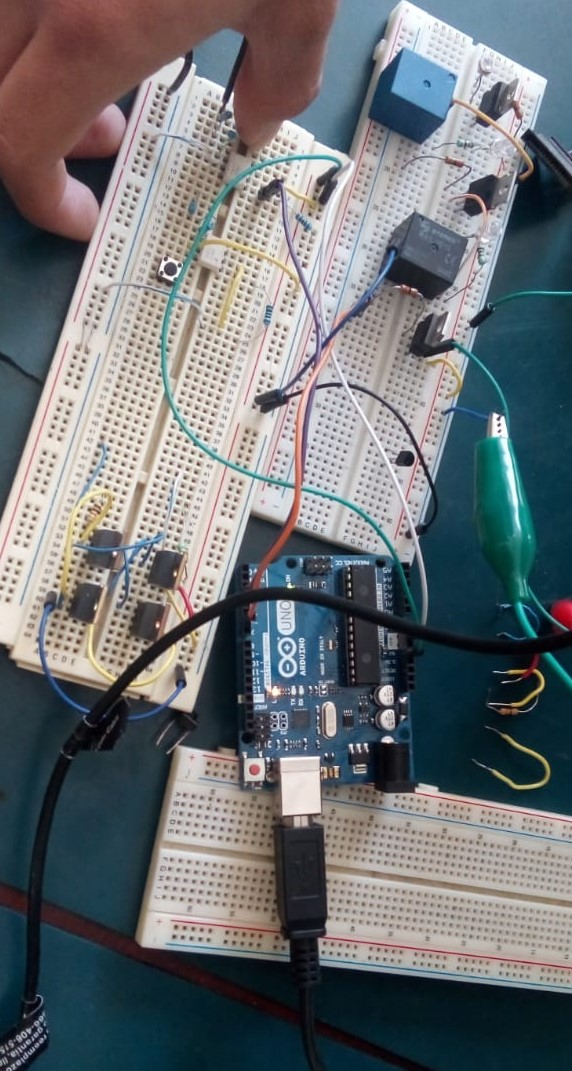
\includegraphics[scale=0.3]{Pictures/Relevador.jpeg}
\caption{Circuito de activación Relevador Industrial}
\end{figure}

Conecta las fuentes y activa el push button y esto es lo que sucede: \\
\begin{figure}[hbtp]
\centering
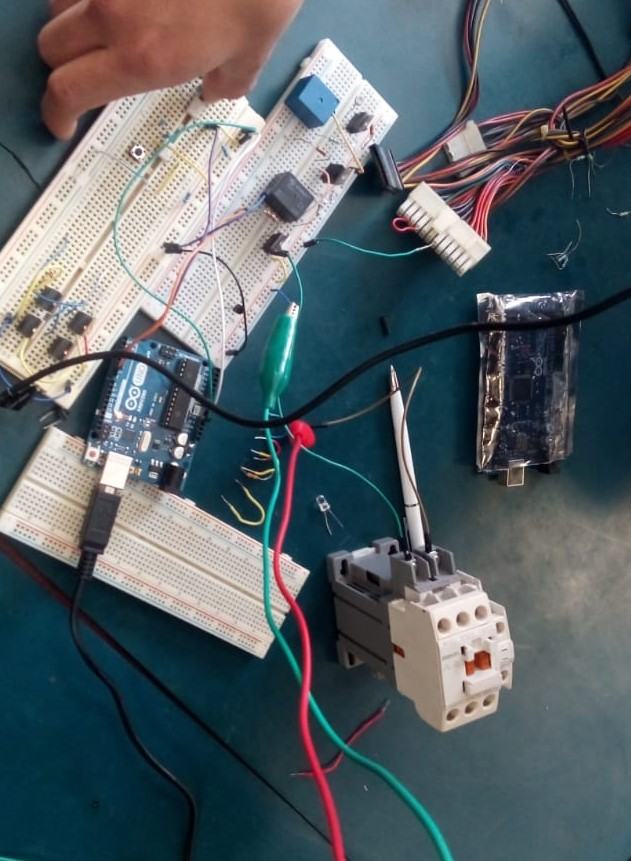
\includegraphics[scale=0.3]{Pictures/Industrial.jpeg}
\caption{Activación del Relevador Industrial}
\end{figure}

Observamos que el relevador industrial se activa mediante el Darlington y 24V dados por una fuente de alimentación.

\footnote{Universidad Politécnica de la Zona Metropolitana de Guadalajara}
 
\newpage
\subsection{Activación del Darlington mediante un LDR}
Teniendo el siguiente circuito vamos a lograr encender un Led mediante un LDR:
\begin{figure}[hbtp]
 \centering
 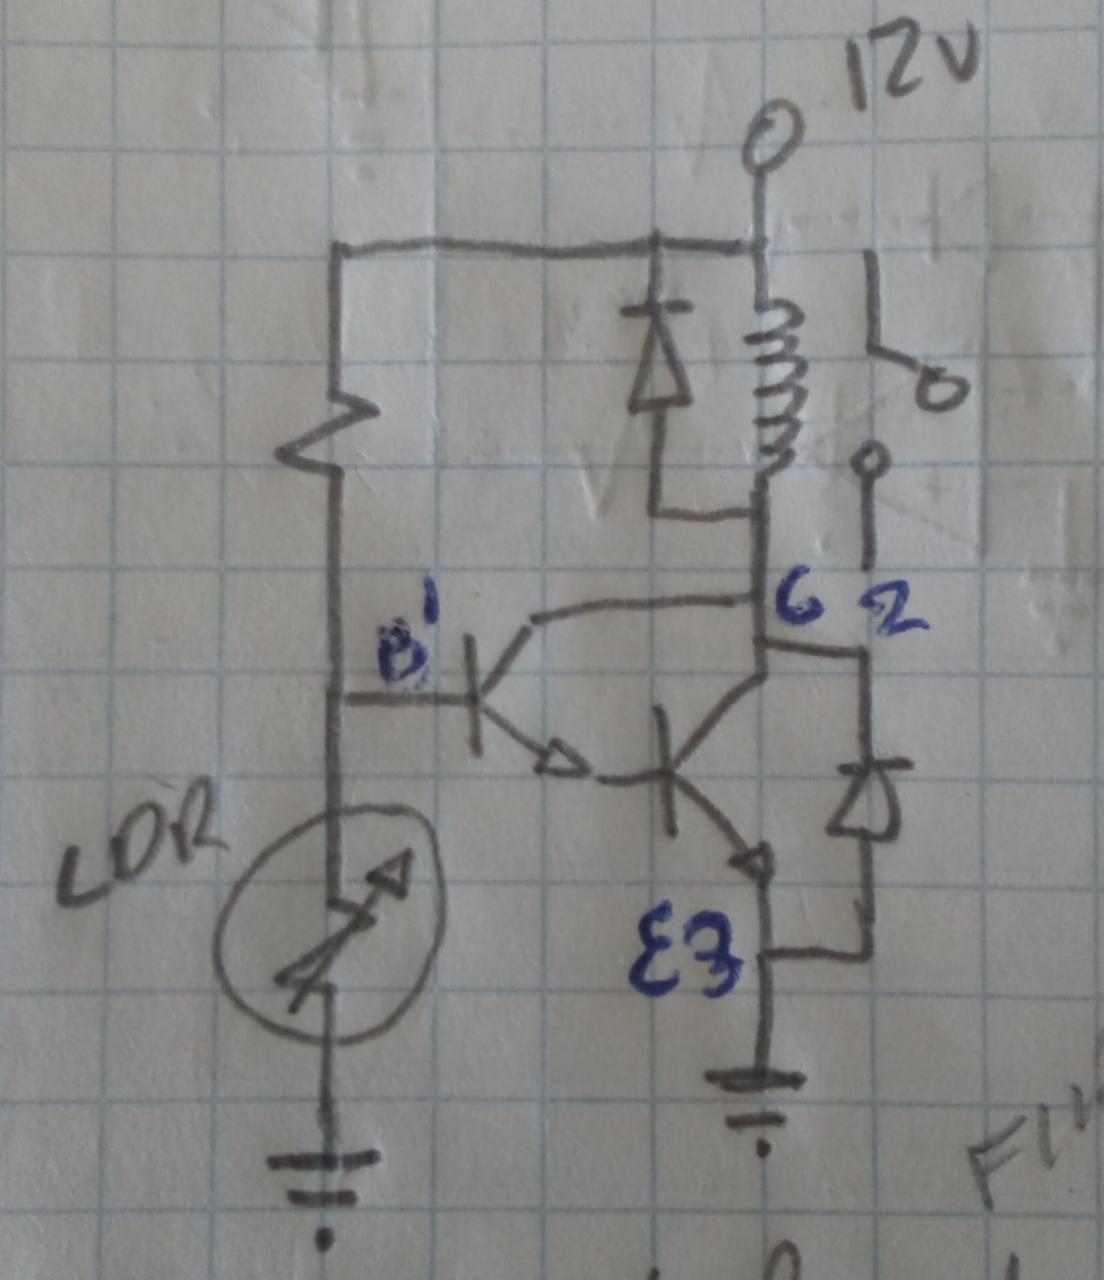
\includegraphics[scale=0.1]{Pictures/LDRA.jpeg}
 \caption{Circuito activacón Darlington con LDR}
 \end{figure}
  
Vamos a armar el circuito en protoboard para poder ver el funcionamiento y la activación del Darlington, quedando el circuito armado: 
\begin{figure}[hbtp]
\caption{Circuito LDR armado}
\centering
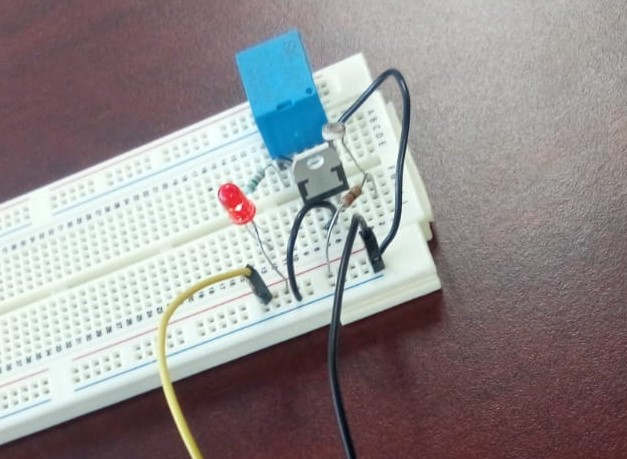
\includegraphics[scale=0.4]{Pictures/LDR.jpeg}
\end{figure}

Conectamos la fuente de voltaje en 5V y observamos lo que ocurre: 
\begin{figure}[hbtp]
\centering
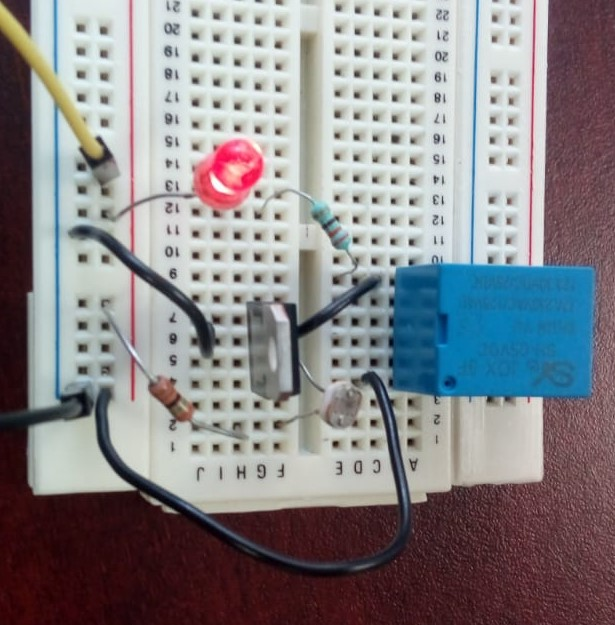
\includegraphics[scale=0.4]{Pictures/LDR1.jpeg}
\caption{Activación LDR}
\end{figure}
\footnote{Universidad Politécnica de la Zona Metropolitana de Guadalajara}

\newpage
 Observamos que el LED enciende y el relevador se activa, ahora lo único que debemos de hacer es taparle la luz para que se desactive y se apague el LED, como se muestra a continuación: 
 \begin{figure}[hbtp]
 \centering
 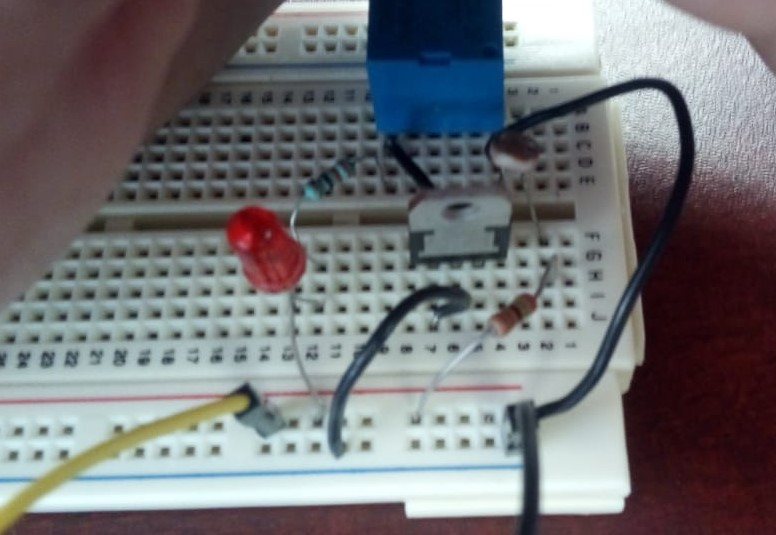
\includegraphics[scale=0.4]{Pictures/LDR2.jpeg}
 \caption{Desctivación LDR}
 \end{figure}
 
\section{Conclusiones}
Para está práctica no se nos dificulto para nada, simplemente realizamos tal cual nos la pidieron y se logró la única en la que tuvimos problema fue en el relevador industrial ya que no se activaba, duramos más de una hora tratando en activarlo, y al final de la clase se logró realizarlo mediante un despeje, tuvimos que tomar tierra de otra fuente a nuestra tierra del circuito y así funcionó a la perfección. \\

La función del LDR es activarse o desactivarse al contacto con la luz, en nuestro caso se activa con la luz y se desactivó cuando nosotros le tapamos la luz, logrando encender el LED y el relevador.\\

La activación del Darlington se logró mediante el arduino y una resistencia de 1.5k$\Omega$ y logró encender el relevador de 5V y el relevador industrial de 24V. El Darlington se usa más en las industrias para manejar voltajes más elevados.\\

El manejo del Darlington es sumamente diferente al utilizado en la práctica 2, el Transistor 2N2222 cambia su estructura y la estructura del Darlington es el doble del 2n2222 y tiene incluido un diodo, esto facilita el uso de voltajes mas altos.\\

\footnote{Universidad Politécnica de la Zona Metropolitana de Guadalajara}

\newpage
\section{Referencias bibliográficas}

\url{https://www.ecured.cu/Transistor_Darlington}

\begin{figure}[hbtp]
\centering
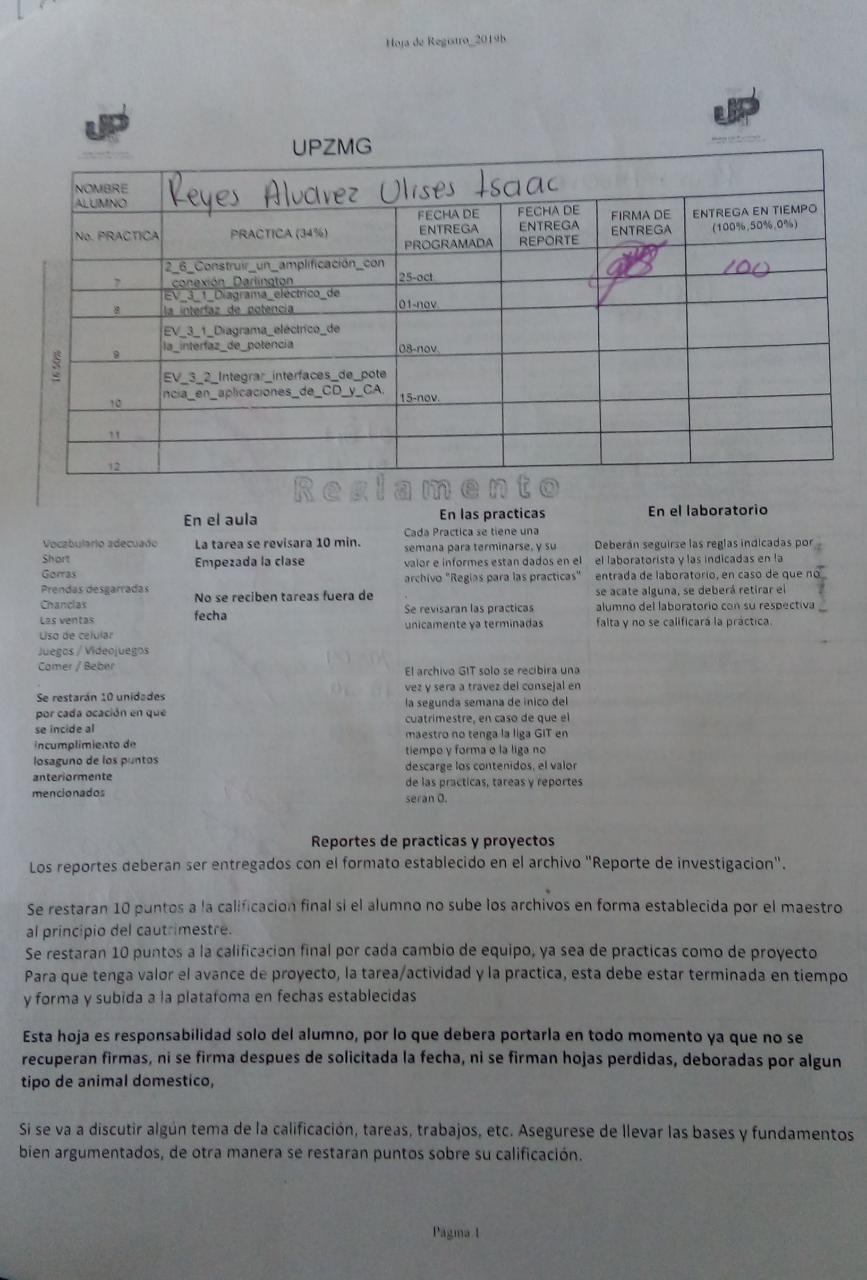
\includegraphics[scale=0.43]{Pictures/Firma.jpeg}
\end{figure}

\footnote{Universidad Politécnica de la Zona Metropolitana de Guadalajara}

\end{document}